\documentclass[sigconf]{acmart}
\usepackage{booktabs} \usepackage{multirow}

\settopmatter{printacmref=false, printccs=false, printfolios=true}
\renewcommand\footnotetextcopyrightpermission[1]{}

\usepackage{listings}
\usepackage{graphicx}
\usepackage{float}
\usepackage[T1]{fontenc}

\begin{document}
    \lstset{language=bash}
    \title{Iterative Histogram Equalization}
    \subtitle{Concurrency and Parallelism 2023-24}



    \author{Francisco Vasco}
    \email{f.vasco@campus.fct.unl.pt}

    \author{Tomé Dias}
    \email{td.dias@campus.fct.unl.pt}


    \begin{abstract}
        In this project we study, apply and test different parallelization approaches over the iterative histogram equalization algorithm and their performance.
        We implement parallel versions of the algorithm using both OpenMP and CUDA.
    \end{abstract}

    \keywords{iterative histogram equalization, OpenMP, CUDA, parallel computing, image processing}

    \maketitle

    \section{Evaluation Setup}.
    For this section we present the hardware, software and evaluation methodology used in our experiments.

    \subsection{Hardware}

    \begin{itemize}
        \item \textbf{CPU:} AMD Ryzen 7 7840HS @ 3.80 GHz (up to 5.10 GH (8 cores, 16 threads)
        \item \textbf{GPU:} NVIDIA GeForce RTX 4060 (8GB GDDR6)
        \item \textbf{RAM:} 16GB (2*8GB) DDR5-5600MHz
        \item \textbf{Storage:} 500GB SanDisk Extreme SSD Portatil
    \end{itemize}

    \subsection{Software}

    \begin{itemize}
        \item \textbf{Operating System:} Ubuntu 24.04 (64-bit)
        \item \textbf{Compiler:} GCC 13.2.0
        \item \textbf{CUDA Toolkit:} Version 12.0
        \item \textbf{OpenMP:} Enabled with GCC
        \item \textbf{Libraries:}
        \begin{itemize}
            \item googlebenchmark 1.8.4
            \item googletest 1.14.0
        \end{itemize}
    \end{itemize}

    \subsection{Benchmark Setup}
    Each benchmark was conducted under the following conditions:
    \begin{itemize}
        \item No other significant processes were running during the benchmarks to minimize resource contention.
        \item For each configuration (number of iterations, image size) we calculated the average times for the different implementations, and the average results were reported.
        \item The images used for testing were of different resolutions: 512x512, 1024x1024, 2048x2048, 4096x4096, 8192x8192,

        12288x12288.
    \end{itemize}

    \subsection{Commands}
    To create the images used for our testing purposes first run the script inside the \verb|scripts| folder:

    \begin{lstlisting}
sh gen_images.sh
    \end{lstlisting}

    Afterwards compile and build the project by simply running the commands initially used in the project from the project's root directory:

    \begin{lstlisting}
mkdir build
cd build
cmake ..
make
    \end{lstlisting}

    To run the benchmarks used for assessing the performance of our solutions run:

    \begin{lstlisting}
benchmarking/bm_target
    \end{lstlisting}

    \section{Stage 1}
    Initially we analyzed the source code to have a better understanding about how the program works.

    Then we divided the code in functions we thought were similar and could be parallelized.

    We ran a Profiler on the code in order to identify potential hot-spots and bottlenecks.

    The first thing we identified was the use of std::sharedptr, and we found that it was much faster to use default pointers and deal with the freeing of memory on our own.

    With the professor's feedback we also found a way to join two for loops in one and erase the gray image array.

    We found that using a reduction was a good way to deal with concurrency as it creates various copies of the histogram and adds them together at the end, saving the system a lot of time at the cost of a small amount of memory.

    Due to the size of the CDF we found that there was no need to parallelize the for loop that fills it as it is basically impossible to parallelize due to the true dependency present.

    After running the Profiler multiple times, and dealing with some minor mistakes, we decided that we had reached the full potential of the parallelization.

    We then wrote some basic benchmarks to evalute our code and the Stage 1 was considered done.


    \section{Stage 2}
    Since we already knew from previous profiling and analysis for stage 1 what we should parallelize we applied the same methodology this time using the stage 1 code as the base for our implementation and did each for loop as one CUDA function.

    Initially we were copying all the arguments to the GPU before each function but we found that there was no need for that as we could re-use the ones that were already there, and that saved us a lot of execution time due to reduced data transfers between host and device.

    We also found errors in our testing for equal results between the stage 1 version and our CUDA version, due to differences in implementation of floating point operations between the host and the device, so we decided to test correctness using a +/- 0,03 error margin to account for floating point errors.

    In the end it was basically implementing the CUDA functions and the parallelization was complete.

    \section{Profiling}
    From what we observed from profiling the sequential version \ref{fig:seqprofile}, most of the runtime was taken up by these functions called by the histogram equalization function (59.97\%) for each iteration: \begin{lstlisting}
fill_with_correct_color (26.8%),
fill_output (12.7%)
init_image_arr (8.4%)
calculate_rgb (6.2%)
    \end{lstlisting}
    For the parallel OpenMP version \ref{fig:parprofile} we observed significant improvements by combining the \textit{fill{\_}with{\_}correct{\_}color} and \textit{fill{\_}output} into one function, \textit{apply{\_}cdf}, and by parallelizing the \textit{calculate{\_}rgb} function.
    For the CUDAversion \ref{fig:cudaprofile} most of the runtime was taken by the memory transfers between host and device, kernel system calls and processing on the GPU's end.


    \section{Performance Analysis}
    Through our experiments we observed that the parallel OpenMP implementation of the algorithm using 8 workers consistently achieved a speedup around 6-7x , as seen in Table \ref{tab:benchmark}, compared to the sequential implementation while the CUDA implementation also showed significant speedups, especially as the image size and number of iterations increases, reaching speedups of 60.97x. Conversely, it did not perform as well as the OpenMP version for the smaller images with fewer iterations due to the cost of memory transfers between host and device which becomes less noticeable for larger workloads (increased size and iterations).
    It is also interesting to see that for images of size 8192x8192 or larger the execution times for equalization with more than 1 iteration remained similar across different number of iterations.

    \section{Individual Contributions}
    The contributions to the project for each member were the following:

    \subsection{Francisco Vasco}
    \begin{itemize}
        \item \textbf{CMake Configuration:} 70\%
        \item \textbf{OpenMP Implementation:} 30\%
        \item \textbf{CUDA Implementation:} 40\%
        \item \textbf{Benchmarking:} 60\%
        \item \textbf{Profiling:} 50%
        \item \textbf{Report:} 60%
    \end{itemize}

    \subsection{Tomé Dias}
    \begin{itemize}
        \item \textbf{CMake Configuration:} 30\%
        \item \textbf{OpenMP Implementation:} 70\%
        \item \textbf{CUDA Implementation:} 60\%
        \item \textbf{Benchmarking:} 40\%
        \item \textbf{Profiling:} 50%
        \item \textbf{Report:} 40%
    \end{itemize}


    \begin{table}[h]
        \caption{Benchmark Results for Different Image Sizes and Iterations}
        \label{tab:benchmark}
        \resizebox{\columnwidth}{!}{%
            \begin{tabular}{ccccccc}
                \hline
                \multirow{2}{*}{\textbf{\begin{tabular}[c]{@{}c@{}}Image\\ Size\end{tabular}}} &
                \multirow{2}{*}{\textbf{\begin{tabular}[c]{@{}c@{}}Number of \\ Iterations\end{tabular}}} &
                \multicolumn{3}{c}{\textbf{Time (ms)}} &
                \multicolumn{2}{c}{\textbf{Speedup}} \\ \cline{3-7}
                &
                &
                \textbf{Sequential} &
                \textbf{OpenMP} &
                \textbf{CUDA} &
                \multicolumn{1}{l}{\textbf{OpenMP}} &
                \multicolumn{1}{l}{\textbf{CUDA}} \\ \hline
                \multirow{4}{*}{512x512}                         & 1  & 7.37  & 1.15  & 2.68    & 6.42 & 2.75                     \\ \cline{2-7}
                & 5  & 35.9  & 5.45  & 8.10    & 6.59 & 4.43                     \\ \cline{2-7}
                & 10 & 71.8  & 11.0  & 12.91   & 6.53 & 5.56                     \\ \cline{2-7}
                & 20 & 143   & 21.5  & 25.6    & 6.65 & 5.58                     \\ \hline
                \multirow{4}{*}{1024x1024}                       & 1  & 32    & 4.94  & 8.09    & 6.48 & 3.96                     \\ \cline{2-7}
                & 5  & 143   & 22.4  & 26.89   & 6.38 & 5.32                     \\ \cline{2-7}
                & 10 & 284   & 49.6  & 39.16   & 5.73 & 7.25                     \\ \cline{2-7}
                & 20 & 574   & 97.9  & 79.82   & 5.86 & 7.19                     \\ \hline
                \multirow{4}{*}{2048x2048}                       & 1  & 139   & 27.2  & 32.44   & 5.11 & 4.28                     \\ \cline{2-7}
                & 5  & 620   & 105   & 93.29   & 5.90 & 6.65                     \\ \cline{2-7}
                & 10 & 1222  & 176   & 167.12  & 6.94 & 7.31                     \\ \cline{2-7}
                & 20 & 2422  & 347   & 308.28  & 6.98 & 7.86                     \\ \hline
                \multicolumn{1}{l}{\multirow{4}{*}{4096x4096}}   & 1  & 579   & 86.6  & 135.56  & 6.69 & 4.27                     \\ \cline{2-7}
                \multicolumn{1}{l}{}                             & 5  & 2492  & 339   & 355.92  & 7.35 & 7.00 \\ \cline{2-7}
                \multicolumn{1}{l}{}                             & 10 & 4947  & 652   & 635.97  & 7.59 & 7.56                     \\ \cline{2-7}
                \multicolumn{1}{l}{}                             & 20 & 9444  & 1308  & 780.01  & 7.22 & 12.11                    \\ \hline
                \multicolumn{1}{l}{\multirow{4}{*}{8192x8192}}   & 1  & 2138  & 345   & 534.62  & 6.20 & 4.00                     \\ \cline{2-7}
                \multicolumn{1}{l}{}                             & 5  & 9305  & 1357  & 978.12  & 6.86 & 9.51                     \\ \cline{2-7}
                \multicolumn{1}{l}{}                             & 10 & 18254 & 2640  & 996.57  & 6.91 & 18.31                    \\ \cline{2-7}
                \multicolumn{1}{l}{}                             & 20 & 36123 & 5161  & 993.46  & 7.00 & 36.36                    \\ \hline
                \multicolumn{1}{l}{\multirow{4}{*}{12288x12288}} & 1  & 4884  & 983   & 1188.92 & 4.97 & 4.11                     \\ \cline{2-7}
                \multicolumn{1}{l}{}                             & 5  & 20999 & 3157  & 1351.23 & 6.65 & 15.54                    \\ \cline{2-7}
                \multicolumn{1}{l}{}                             & 10 & 40992 & 5918  & 1352.73 & 6.93 & 30.30                    \\ \cline{2-7}
                \multicolumn{1}{l}{}                             & 20 & 81660 & 11890 & 1339.45 & 6.87 & 60.97                    \\ \hline
            \end{tabular}%
        }
    \end{table}

    \appendix
    \begin{figure*}
        \centering
        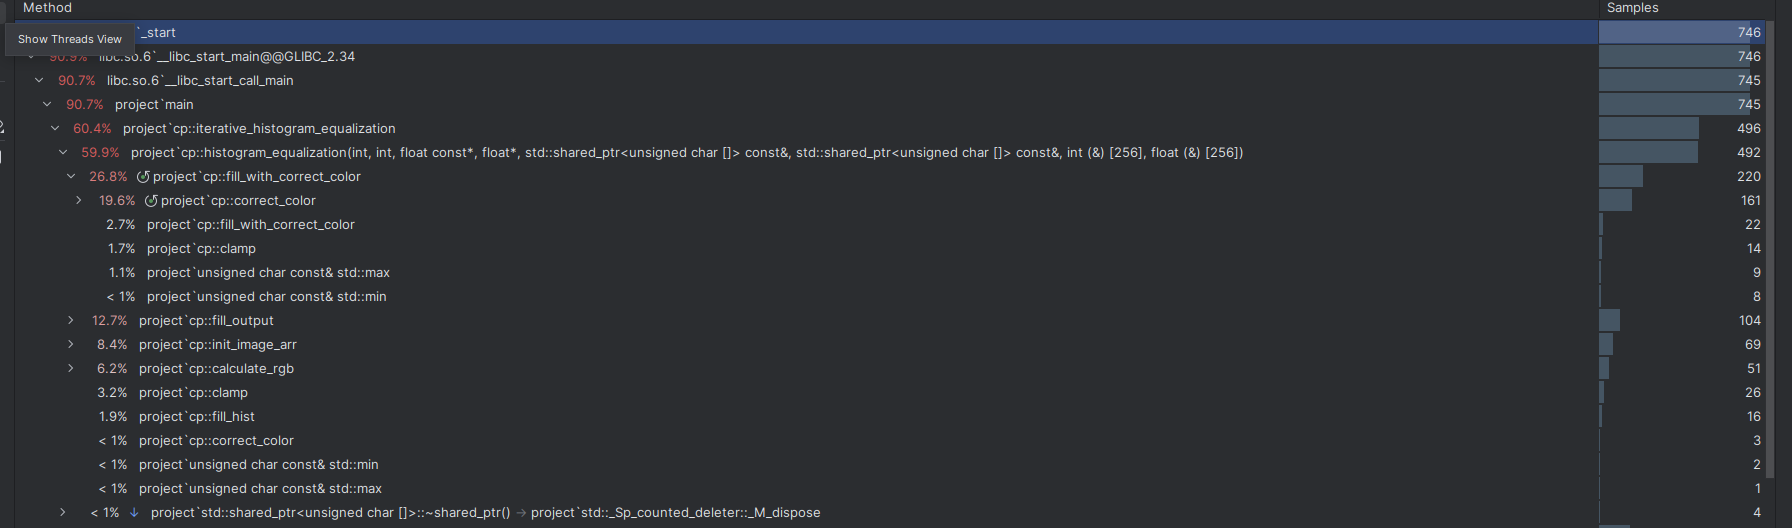
\includegraphics[width=\linewidth]{seqprofile.png}
        \caption{Sequential Profile}
        \label{fig:seqprofile}
    \end{figure*}

    \begin{figure*}
        \centering
        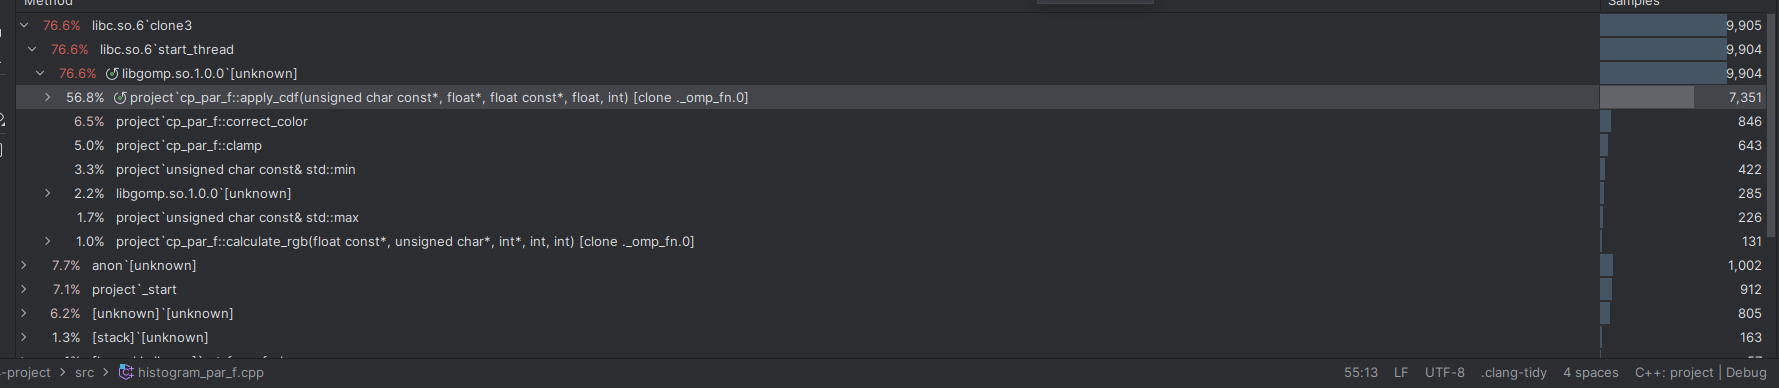
\includegraphics[width=\linewidth]{parprofile.png}
        \caption{Parallel Profile}
        \label{fig:parprofile}
    \end{figure*}

    \begin{figure*}
        \centering
        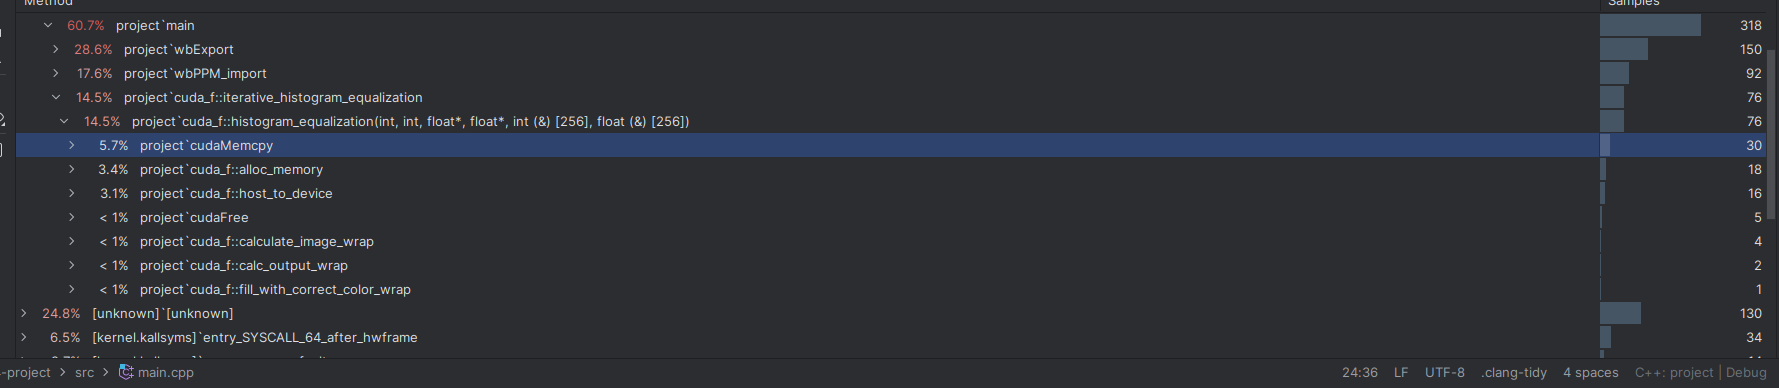
\includegraphics[width=\textwidth]{cudaprofile.png}
        \caption{CUDA Profile}
        \label{fig:cudaprofile}
    \end{figure*}

    \bibliographystyle{acm}
    \bibliography{res}

\end{document}